\exercise

Given the suffix tree for the string ``{\tt babacbababad}'' and assume that the
prefix ``{\tt babac}'' has been already LZ-parsed, show how the suffix tree can
be used to execute the next LZ-parsing step (i.e., the identification of the
next LZ-phrase) in an efficient way.

\solution

\autoref{fig:lz77-suffix-tree} show the suffix tree of the given string.
%
\begin{figure}[t]
  \centering
  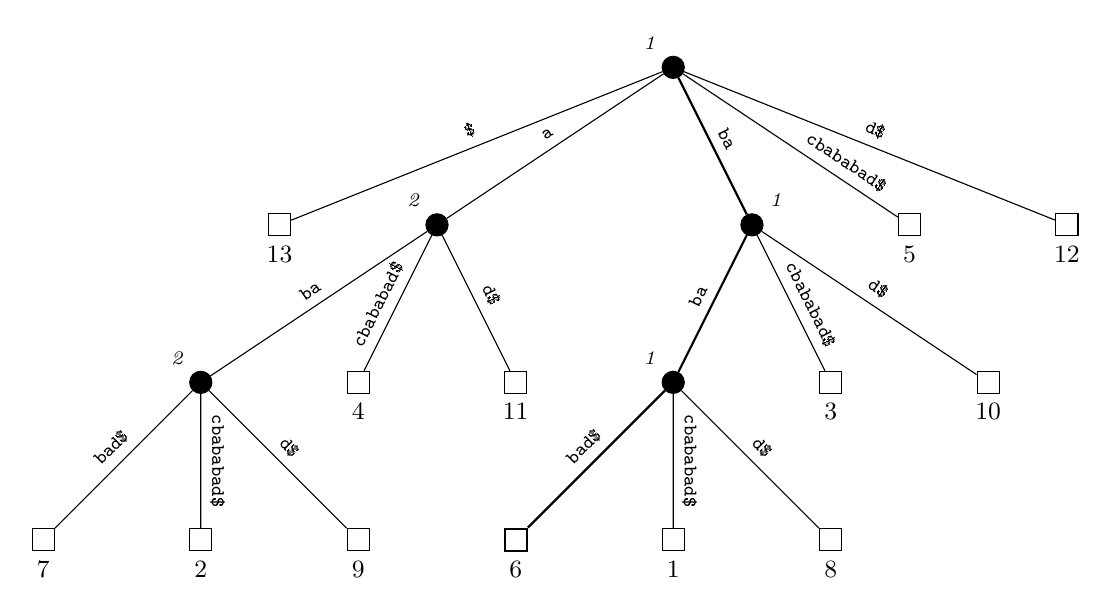
\begin{tikzpicture}[
    grow=down,
    inner/.style={thin, draw, fill, inner sep=0, minimum size=8, circle},
    leaf/.style={thin, draw, fill=white, inner sep=0, minimum size=8},
    phantom/.style={draw=none, fill=none},
    level 1/.style={sibling distance = 2cm,level distance = 2cm},
    level 2/.style={sibling distance = 2cm, level distance = 2cm},
    level 3/.style={sibling distance = 2cm, level distance = 2cm},
    every edge/.style={-, thin}
  ]
  \node[inner, label=above left:{\scriptsize\it 1}] {}
  child {
    node[leaf, label=below:{\small 13}] {}
    edge from parent[-] node[above, sloped] {\scriptsize\tt \$}
  }
  child {
    node[inner, label=above left:{\scriptsize\it 2}] {}
    child {
      node[inner, label=above left:{\scriptsize\it 2}] {}
      child {
        node[leaf, label=below:{\small 7}] {}
        edge from parent[-] node[above, sloped] {\scriptsize\tt bad\$}
      }
      child {
        node[leaf, label=below:{\small 2}] {}
        edge from parent[-] node[above, sloped] {\scriptsize\tt cbababad\$}
      }
      child {
        node[leaf, label=below:{\small 9}] {}
        edge from parent[-] node[above, sloped] {\scriptsize\tt d\$}
      }
      edge from parent[-] node[above, sloped] {\scriptsize\tt ba}
    }
    child {
      node[leaf, label=below:{\small 4}] {}
      edge from parent[-] node[above, sloped] {\scriptsize\tt cbababad\$$\quad$}
    }
    child {
      node[leaf, label=below:{\small 11}] {}
      edge from parent[-] node[above, sloped] {\scriptsize\tt d\$}
    }
    child {
      node[phantom] {}
      edge from parent[draw=none]
    }
    edge from parent[-] node[above, sloped] {\scriptsize\tt a}
  }
  child {
    node[phantom] {}
    edge from parent[draw=none]
  }
  child {
    node[inner, label=above right:{\scriptsize\it 1}] {}
    child {
      node[phantom] {}
      edge from parent[draw=none]
    }
    child {
      node[inner, label=above left:{\scriptsize\it 1}] {}
      child {
        node[leaf, thick, label=below:{\small 6}] {}
        edge from parent[-, thick] node[above, sloped] {\scriptsize\tt bad\$}
      }
      child {
        node[leaf, label=below:{\small 1}] {}
        edge from parent[-, thin] node[above, sloped] {\scriptsize\tt cbababad\$}
      }
      child {
        node[leaf, label=below:{\small 8}] {}
        edge from parent[-, thin] node[above, sloped] {\scriptsize\tt d\$}
      }
      edge from parent[-, thick] node[above, sloped] {\scriptsize\tt ba}
    }
    child {
      node[leaf, label=below:{\small 3}] {}
      edge from parent[-, thin] node[above, sloped] {\scriptsize\tt $\quad$cbababad\$}
    }
    child {
      node[leaf, label=below:{\small 10}] {}
      edge from parent[-, thin] node[above, sloped] {\scriptsize\tt d\$}
    }
    edge from parent[-, thick] node[above, sloped] {\scriptsize\tt ba}
  }
  child {
    node[leaf, label=below:{\small 5}] {}
    edge from parent[-] node[above right, sloped] {\scriptsize\tt cbababad\$}
  }
  child {
    node[leaf, label=below:{\small 12}] {}
    edge from parent[-] node[above, sloped] {\scriptsize\tt d\$}
  };
  \end{tikzpicture}

  \caption{Suffix tree for the word ``{\tt babacbababad\$}''. The labels over
  the inner nodes (in italic) represent the minimum value among the leaves of
  their subtrees. The thick path represents the suffix to be parsed, $\text{\it
  suff}_6 = \text{\tt bababad\$}$.}

  \label{fig:lz77-suffix-tree}
\end{figure}
%
To compute the next LZ-parsing step, we need to preprocess the suffix tree such
that every node contains the value of the minimal leaf in its subreee. This can
be done in linear time using a post-order visit (i.e., for each each children of
a node, compute their minimum recursively). This value represents the leftmost
suffix that shares the same prefix of all the other leaves in the subtree. With
this information, the next LZ token starting from $\text{\it suff}_i$ can be
computed by taking the lowest label $j$ in the downpath of $\text{\it suff}_i$
such that $j < i$. In this case, given $i = 6$, the lowest inner node $u$ has
value $j = 1 < i$. The next LZ token is $\langle i - j, \ell, \text{\it
suff}_i[\ell + 1] \rangle = \langle 5, 4, {\tt b} \rangle$, where $\ell$ is the
length of the string spelled by node $u$.
